\chapter{Introduction}



\section{Motivation}

%TODO: Make this prettier
\begin{figure}[ht!]
  \centering
    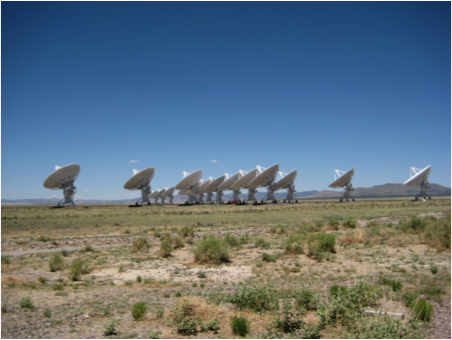
\includegraphics[width=0.49\textwidth]{Images/C1/vla.png}
    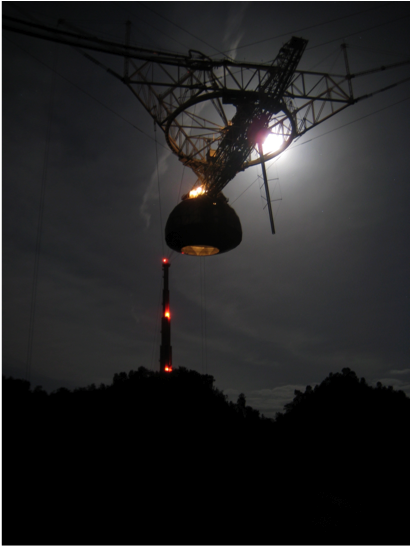
\includegraphics[width=0.49\textwidth]{Images/C1/arecibo.png}
    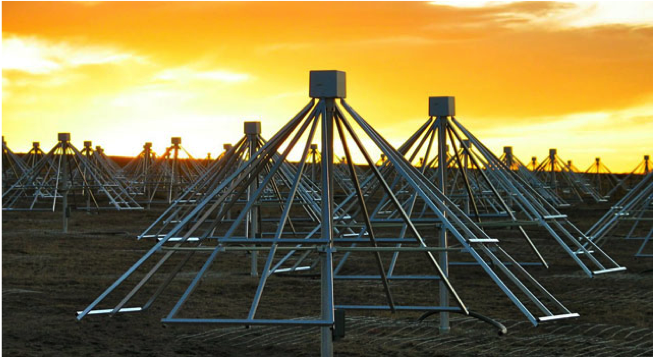
\includegraphics[width=0.49\textwidth]{Images/C1/paper.png}
  \caption{TODO Telescopes}
  \label{fig: C1/telescopes}
\end{figure}


%TODO: Make this prettier, maybe add a graphic
\begin{figure}[ht!]
  \centering
    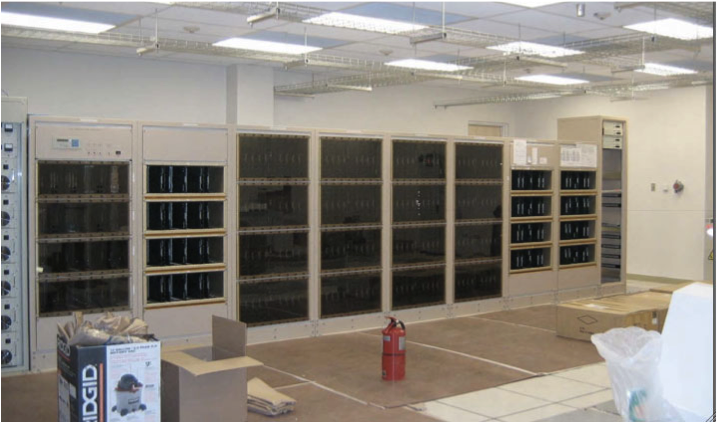
\includegraphics[width=0.49\textwidth]{Images/C1/alma_correlator.png}
    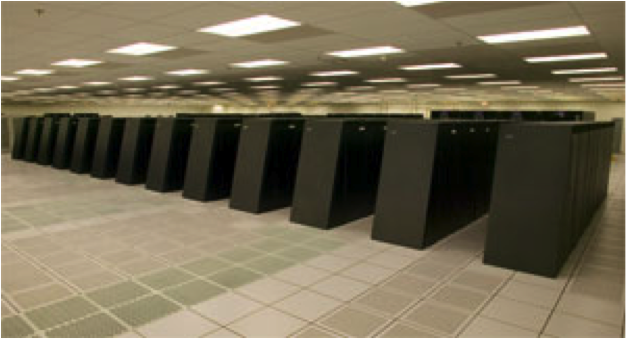
\includegraphics[width=0.49\textwidth]{Images/C1/blue_gene.png}
    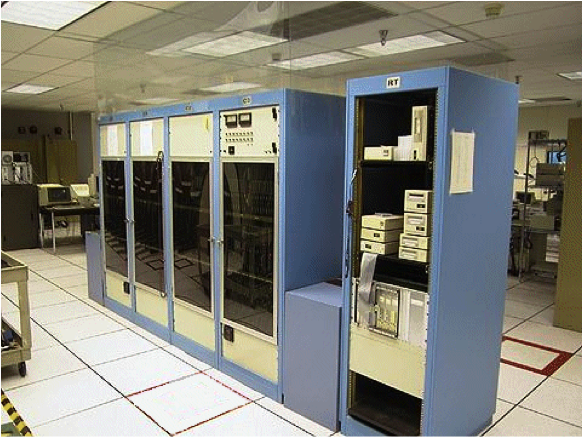
\includegraphics[width=0.49\textwidth]{Images/C1/vla_correlator.png}
  \caption{TODO Building large systems}
  \label{fig: C1/largesystems}
\end{figure}

%TODO: add some references

\begin{figure}[ht!]
  \centering
    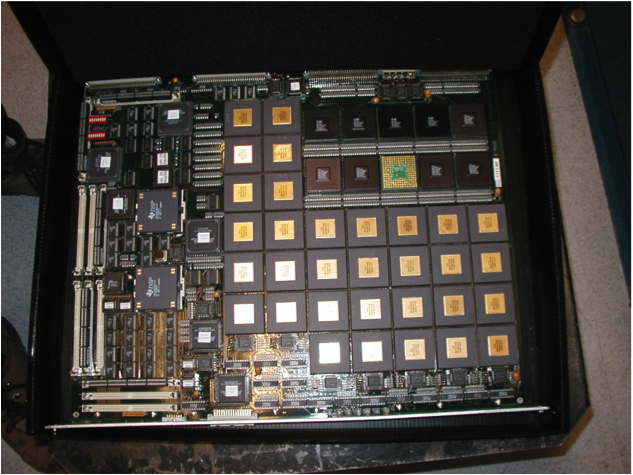
\includegraphics[width=0.49\textwidth]{Images/C1/custom_asic.png}
    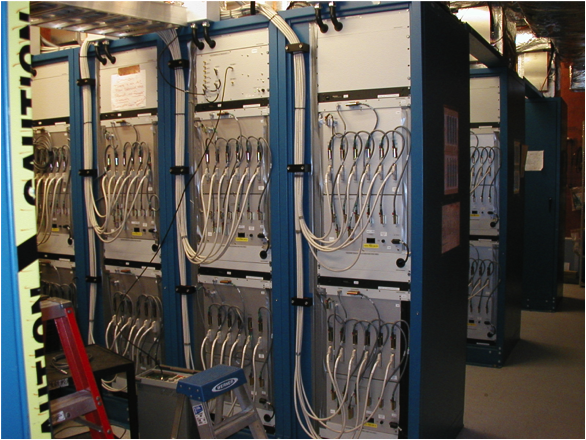
\includegraphics[width=0.49\textwidth]{Images/C1/custom_interconnect.png}
  \caption{TODO Building large systems}
  \label{fig: C1/largesystems}
\end{figure}

Traditionally, observatories designed custom instruments that would run on one telescope and solve one problem.
This custom approach was the only way to get the requisite processing power to analyze the radio signals, but it resulted in costly designs, because the boards, backplanes, chips, protocols, and software all needed to be designed from scratch.
To make matters worse, this approach resulted in a very long design cycle,  requiring 5-10 years of development before an instrument could be deployed at a telescope and the time the instrument was released, the hardware would be out of date.

Due to their custom implementations, these instruments also lacked flexibility. 
Each instrument was designed specifically for a single purpose.
A hardware upgrade or algorithm modification would require a complete redesign of the instrument, and another long design cycle.


While these older designs needed to trade off flexibility for performance, newer technology can offer both performance and flexibility.
Programmable devices such as FPGAs, GPUs and even CPUs can provide enough processing power to keep up with the data from many new telescopes.
These devices make it easy to reprogram existing hardware to support newer algorithms, and, since they are programmed using portable languages, provide a quick path to upgrade hardware without redesigning the entire instrument.


%We implement the instrument on a heterogeneous cluster consisting of both FPGAs and GPUs to take advantage of the benefits provided by both platforms.
%FPGAs provide high bandwidth processing but can be cumbersome to program.
%GPUs can't handle the same bandwidths as FPGAs but they are easier to program. 
%The CUDA language, for example, is a C-like language that can be used to develop software for many GPUs.
%The high level parameters in this package allow us to use FPGAs while abstracting away implementation details specific to the FPGA.
%To give the user control over their data processing algorithm, an application specific GPU program can be written and easily interfaced with the existing receive software in the package.

%The instruments generated with this package use a heterogeneous design, allowing us to benefit from the strengths of FPGAs and GPUs. 
%The FPGA board is able to sample and process very high bandwidths that a single CPU or GPU would not be able to manage; 
%once the FPGA has split up the band the GPU provides a platform that is easier than an FPGA to program but still provides high compute power. 
%A design called the Packetized Astronomy Signal Processor, or PASP, is run on the FPGA.
%PASP splits up the large band into smaller bands that can be processed using off the shelf servers.
%The subbands are put into packets on the FPGA and sent over a 10 gigabit Ethernet switch to a cluster of servers.
%The servers receive the data from the switch and process it using spectroscopy software provided in the software package or special purpose application software written by the user and linked into the provided packet processing infrastructure.

\section{Challenges}

\subsection{Scientific Challenges}
Radio astronomers are trying to answer a very diverse set of questions. 
%Let�s think about what we�re actually trying to do
%Deal with a diverse set of questions
%Are we alone?
%When were the first stars and galaxies formed?
%Galactic structure and formation (mapping the galaxy)
%Nature of gravitational wave background (pulsar timing)
%Transient universe
%Black hole imaging
%Searching for extrasolar planets

%Number of antennas
%Bandwidth
%Number of channels
%Filter shapes
%Integration time
%Algorithms
%Etc�

%Spectrometer
%Beamformer
%Add signals from multiple antennas together to improve SNR
%Pulsar processor
%Detect dispersed pulse
%Interferometer/correlator
%Cross-correlate signals from many antennas to combine into a spectral image
%Increase angular resolution

%Spectrometer
%Filter bank/FFT
%Accumulation
%Beamformer
%FFT
%Phase shift
%Adders
%Pulsar processor
%FFT
%Deconvolution
%Interferometer/correlator
%FFT
%Cross correlation (multipliers)
%Accumulation

\subsection{Technological Challenges}

%Large number of small antennas to improve sensitivity and resolution
%Small antennas are very low cost
%Creates very high performance signal processing requirements
%Need to combine the antennas together to form a single image or beam
%Interferometry computation requirements scale as N2 (N = number of antennas) ~100Tops

\begin{figure}[ht!]
  \centering
    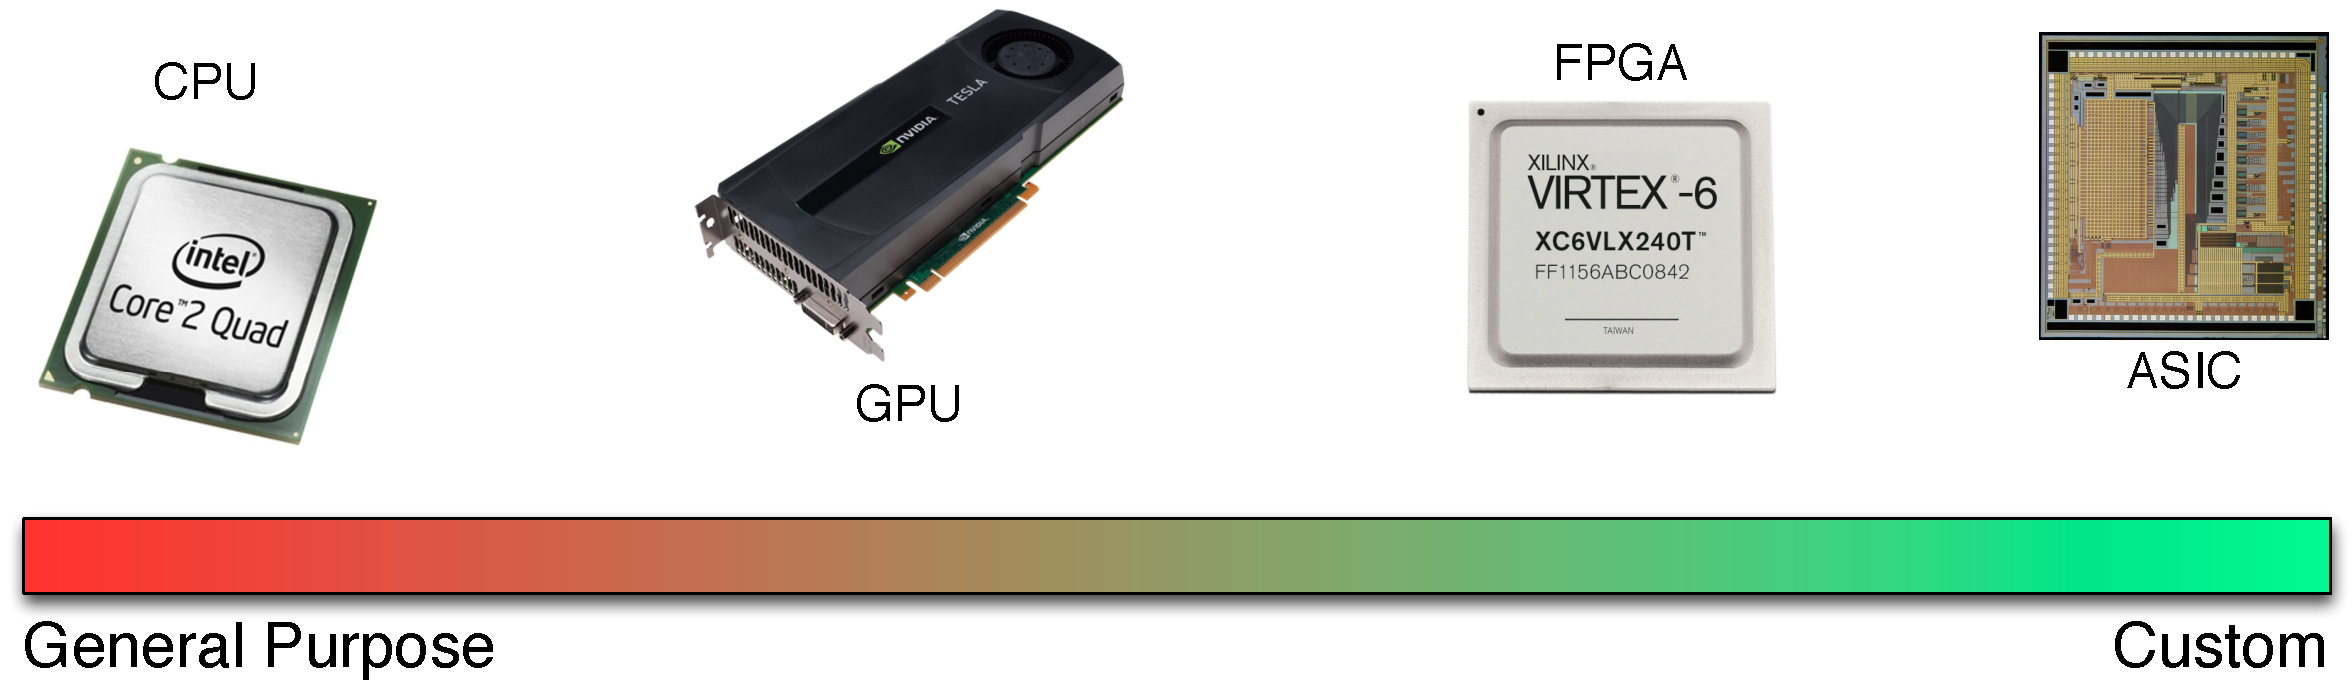
\includegraphics[width=\textwidth]{Images/C1/design_space.pdf}
  \caption{TODO}
  \label{fig: C1/design_space.pdf}
\end{figure}

%Increasing
%
%Design time
%
%Design complexity
%
%Performance
%
%Cost (in low volume)
%
%Decreasing
%
%Power (watts)
%
%Flexibility




%Assessing tradeoffs
%3 GHz bandwidth
%100-200 MHz bandwidth
%Fixed point
%Floating point
%Streaming designs
%Conditional/Iterative programming
%Difficult to program (HDL)
%Easy to program (CUDA)
%Difficult to achieve peak performance
%Difficult to achieve peak performance
%$$
%$
%Lots of available IO
%Limited IO

%Zooming in on the middle of the spectrum, a lot of other things to consider
%Options for reprogrammable architecture
%Floating point can be good or bad depending on the application, some can get away with very small bit widths

%Traditional instrument design
%Traditionally observatories build custom instruments
%High cost due to custom designed 
%boards
%backplanes
%chips 
%protocols
%software
%Development takes 5 to 10 years
%Hardware is out of date by the time it�s released
%Difficult to upgrade/modify without a redesign

%A number of options are available but which is best?
%Need to understand how to choose the right platform(s) for each implementation
%With constant changes in technology and algorithm implementations an automatic approach is required

\section{ORCAS}



